\documentclass[12pt]{article}

\usepackage[utf8]{inputenc}
\usepackage[french]{babel}
\usepackage{graphicx}
\usepackage[left=2cm,right=2cm,top=2cm,bottom=2cm]{geometry}
\usepackage{titlesec}
\usepackage{hyperref}
\usepackage[babel=true]{csquotes}
\usepackage{color} 
\usepackage[T1]{fontenc}
\usepackage{amsmath}
\usepackage{amssymb}
\usepackage{amsthm}
\usepackage{float}
\usepackage{listings}
\usepackage{mathrsfs}
\usepackage{pgfgantt}

\definecolor{linkcolor}{rgb}{0,0,0.3}

\hypersetup{colorlinks,
            citecolor = linkcolor,
            filecolor = linkcolor,
            linkcolor = linkcolor,
            urlcolor = linkcolor}

\theoremstyle{definition}
\newtheorem{definition}{Définition}
\newtheorem{theorem}{Théorème}
\newtheorem{lemma}{Lemme}
\newtheorem{prop}{Propriété}
\newtheorem{exemple}{Exemple}

\titleformat{\part}
  {\normalfont\LARGE\bfseries}{\thepart}{1em}{}
\titlespacing*{\part}{0pt}{3.5ex plus 1ex minus .2ex}{2.3ex plus .2ex}

\newcommand\mycom[2]{\genfrac{}{}{0pt}{}{#1}{#2}}

\setcounter{secnumdepth}{5}
\setcounter{tocdepth}{5}

\lstset{backgroundcolor=\color{white},
  basicstyle=\footnotesize,
  breakatwhitespace=false,
  breaklines=true,
  captionpos=b,
  commentstyle=\color{mygreen},
  deletekeywords={...},
  escapeinside={\%*}{*)},
  extendedchars=true,
  frame=single,
  keepspaces=true,
  keywordstyle=\color{blue},
  language=Python,
  morekeywords={*,...},
  numbers=left,
  numbersep=5pt,
  numberstyle=\tiny\color{mygray},
  rulecolor=\color{black},
  showspaces=false,
  showstringspaces=false,
  showtabs=false,
  stepnumber=5,
  stringstyle=\color{mymauve},
  tabsize=4,
  title=\lstname 
}

%\usepackage{amsfonts}
%\usepackage{lilyglyphs}
%\usepackage{stmaryrd}
%\usepackage{makeidx}
%\makeindex
%\usepackage[english, onelanguage]{algorithm2e}
%\theoremstyle{plain} \newtheorem{prop}{Proposition}

\title{\vspace{20mm}
        \LARGE \textbf {Ordonnancement et équité}\\
        \vspace{8mm}
        \large \textbf{Rapport de stage}\\
        \vspace{10mm}
        \begin{center}
            
\includegraphics[scale = 1]{main_title.jpg}
        \end{center}
        \author{Marion Caumartin}
        \large {Master d'informatique M2}\\
          \vspace{5mm}
        \large {Faculté de Sciences et Ingénieurie de Sorbonne Université \vspace{15mm}}\\ 
        \date{\vspace{10mm} \textsf{\textrm{\textit{6 mars 2019}}}}}



\begin{document}

\maketitle
\thispagestyle{empty}

\newpage

\tableofcontents
\thispagestyle{empty}

\newpage
\setcounter{page}{1}
\section{Introduction}\label{intro}
\noindent
Les problèmes d'ordonnancement constituent un domaine important en recherche opérationnelle. Ils traitent de l'affectation de tâches à des machines, et de l'exécution de ces tâches au cours du temps : il s'agit de savoir où - sur quelle machine - et quand commencera chaque tâche. Récemment, des problèmes d'ordonnancement en présence de différents acteurs ont été étudiés. Cependant, très peu de critères d'équité ont été appliqués aux problèmes d'ordonnancement (hormis le critère classique qui consiste à minimiser le coût maximal d'une machine).\\\\
La théorie du partage équitable est un domaine central en choix social computationnel. Elle s'intéresse à définir des règles d'affectation de ressources à des agents de manière à satisfaire au mieux les agents, sachant que les préférences de ceux-ci peuvent avoir différentes structures inhérentes au problème. Un concept fréquemment utilisé pour évaluer les affectations est celui de l'absence d'envie (envy freeness) : une affectation de ressources est dite sans-envie si aucun des agents ne préfère le lot de ressources d'un autre agent à son propre lot.\\\\
Le but de ce stage est d'appliquer des concepts et techniques développés en théorie du partage équitable, au domaine de l'ordonnancement. On cherche ainsi à évaluer la qualité des ordonnancements du point de vue de l'équité et à calculer des ordonnancements "équitables".

\newpage

\section{Définition du problème}\label{def_pb}

\subsection{Ordonnancement}\label{ordo}

\noindent
On note $m$ le nombre de machines.\\\\
On note $s_i^j$ le slot de temps $i$ de la machine $j$.\\\\
$\lbrace 1,\dots , n \rbrace$ un ensemble d'agents.\\\\
Chaque agent $k$ a un ensemble de $x \in \mathbb{N}$ tâches à réaliser et un critère $f_k$ à minimiser. On note $f_k(s, J)$ le coût du slot pour la tâche $J$ et pour l'agent $k$.\\\\
On note $J_i^k$ la tâche $i$ de l'agent $k$. On note $J^k$ l'ensemble des tâches de l'agent $k$.\\\\
Chaque tâche $J_i^k$ a une durée $p_i^k$, peut avoir une deadline $d_i^k$ et une date de disponibilité $r_i^k$.\\\\
Dans un premier temps, on considère que $\forall k \in \lbrace 1, \dots , n \rbrace, \forall i \in \lbrace 1, \dots , x \rbrace, p_i^k = 1$.\\\\
Un ordonnancement $\sigma$ est définit par les dates de début des tâches : $\sigma(J_i^k)$. On note $\mathscr{S}$ l'ensemble des ordonnancements valides. On note $\sigma(k)$ l'ordonnancement de l'agent $k$ pour l'ordonnancement $\sigma$. On note $\sigma(J^k)$ l'ordonnancement des tâches de $J^k$ pour l'ordonnancement $\sigma$.\\\\
On note $C_i^k$ la date de fin de la tâche $i$ de l'agent $k$ : $C_i^k = \sigma(J_i^k) + p_i^k$.\\\\
$C_{max}^k = \max\limits_i C_i^k$ : date de fin maximum (makespan)\\\\
$T_i^k = \max(0, C_i^k - d_i^k)$ : retard\\\\
$L_i^k = C_i^k - d_i^k$ : retard algébrique\\\\
$U_i^k = \left\{
\begin{array}{l}
  1 \ \mathrm{si} \ C_i^k>d_i^k \\
  0 \ \mathrm{sinon}
\end{array}
\right.$ : vaut 1 si $J_i^k$ est en retard, 0 sinon\\\\
$E_i^k = \max (0, d_i^k - C_i^k)$ : avance\\\\
$S_i^k = (L_i^k)^2$\\\\
$D_i^k = |L_i^k|$

\newpage

\subsection{Equité}\label{equite}

\noindent
On cherche un ordonnancement où chaque agent a exactement $x$ slot : $\forall k \in \lbrace 1, \dots , n \rbrace, |\sigma(k)| = x$.\\\\
$\forall k, k' \lbrace 1, \dots , n \rbrace, \sigma(k)\cap\sigma(k') = \emptyset$.\\\\
Les slots ne peuvent pas être divisés.\\\\
On note $f = (f_1, \dots, f_n)$.\\\\
Pareto-optimalité : $\sigma$ domine $\sigma'$ au sens de Pareto ssi \\
$\left\{
\begin{array}{l}
  \forall k \in \lbrace1, \dots,n\rbrace,f_k(\sigma(k))\leq f_k(\sigma'(k)) \\
  \exists k \in \lbrace1, \dots,n\rbrace,f_k(\sigma(k))< f_k(\sigma'(k))
\end{array}
\right.$\\\\
utilitarian social welfare : minimiser $\sum\limits_{k = 1}^n f_k$.\\\\
egalitarian social welfare : minimiser $\max\limits_{k = 1}^n f_k$.\\\\
leximin : $\sigma \succ_{lex}\sigma' \iff \exists i\in \lbrace1, \dots,n-1\rbrace,
\left\{
\begin{array}{l}
  \forall k < i ,f_k(\sigma(k)) = f_k(\sigma'(k))\\
  f_i(\sigma(i)) < f_i(\sigma'(i))
\end{array}
\right.$\\\\
proportional fair share : on note $f_k^*$ le coût si $k$ disposait des machines pour lui seul.\\ pfs($k$) $ = nf_k^*$.\\\\
maxmin fair share : mfs($k$) $= \min\limits_{\sigma\in\mathscr{S}}\max\limits_{i=1}^n f_k(\sigma(i))$.\\\\
Ordonnancement sans envie : $\forall k,j\in \lbrace1, \dots,n\rbrace, f_k(\sigma(k))\leq f_k(\sigma(j))$\\\\
Envie entre deux agents : $e_{ij} = \max(0, f_i(\sigma(i)) - f_i(\sigma(j)))$\\\\
degré d'envie : $e_i = \max\limits_j e_{ij}$ ou $e_i = \sum\limits_j e_{ij}$\\\\
envie de la société : $\max\limits_i e_i$ ou $\sum\limits_i e_i$\\\\
Envie up to one slot : $i$ envie $j$ up to one slot ssi $\exists s\in \sigma(i), f_i(\sigma(i)\backslash s)\leq f_i(\sigma(j))$\\\\
Envie up to any slot : $i$ envie $j$ up to any slot ssi $\forall s\in \sigma(i), f_i(\sigma(i)\backslash s)\leq f_i(\sigma(j))$\\\\
Envie up to one job : $i$ envie $j$ up to one job ssi $\exists J\in J^i, f_i(\sigma(J^i\backslash J))\leq f_i(\sigma(j))$\\\\
Envie up to any job : $i$ envie $j$ up to any job ssi $\forall J\in J^i, f_i(\sigma(J^i\backslash J))\leq f_i(\sigma(j))$\\\\

\section{Propriétés}
\begin{prop}
    Au moins un ordonnancement egalitarian-optimal est Pareto-optimal.
\end{prop}

\begin{proof}
    Par l'absurde : on suppose qu'il n'existe pas d'ordonnancement egalitarian-optimal et Pareto-optimal.\\
    Soit $\sigma$ un ordonnancement egalitarian-optimal. $\sigma$ n'est donc pas Pareto-optimal. Il existe donc un ordonnancement $\sigma'$ Pareto-optimal qui domine $\sigma$ et qui n'est pas egalitarian-optimal.\\
    2 cas possibles : 
    \begin{itemize}
        \item $\max_{i = 1}^n f_i(\sigma'(i)) = \max_{i = 1}^n f_i(\sigma(i))$ : comme $\sigma$ est egalitarian-optimal, alors $\sigma'$ l'est aussi $\implies$ contradiction.
        \item $\max_{i = 1}^n f_i(\sigma'(i)) \leq \max_{i = 1}^n f_i(\sigma(i))$ : donc $\sigma$ n'est pas egalitarian-optimal $\implies$ contradiction.
    \end{itemize}
\end{proof}

\begin{prop}
    Un ordonnancement sans envie n'est pas toujours Pareto-optimal.
\end{prop}
\begin{exemple}
On considère une instance avec une machine et deux agents $A$ et $B$ qui veulent optimiser le même critère. Chaque agent a deux tâches à exécuter sur la machine. On note $A_i$ (reps. $B_i$) la tâche $i$ de l'agent $A$ (resp. $B$) pour $i \in \lbrace 1,2\rbrace$. Chaque tâche a une deadline : $d_1^A = 1$, $d_2^A = 3$, $d_1^B = 2$ et $d_2^B = 4$.\\
On appelle $\sigma_1$ l'ordonnancement suivant :
\begin{ganttchart}[inline]{1}{8}
    \ganttbar{$A_1$}{1}{2} 
    \ganttbar{$B_1$}{3}{4} 
    \ganttbar{$B_2$}{5}{6} 
    \ganttbar{$A_2$}{7}{8}
\end{ganttchart}\\
On appelle $\sigma_2$ l'ordonnancement suivant :
\begin{ganttchart}[inline]{1}{8}
    \ganttbar{$A_1$}{1}{2} 
    \ganttbar{$B_1$}{3}{4} 
    \ganttbar{$A_2$}{5}{6} 
    \ganttbar{$B_2$}{7}{8}
\end{ganttchart}\\
\begin{itemize}
	\item Si $A$ et $B$ veulent minimiser $\sum T_i$ : $\sigma_1$ est sans-envie mais n'est pas optimal. En effet, $\left\{\begin{array}{l}
	f_A(\sigma_1(A)) = 1 \leq f_A(\sigma_1(B)) = 1\\
	f_B(\sigma_1(B)) = 0 \leq f_B(\sigma_1(A)) = 0
	\end{array}
	\right.$ et $\left\{\begin{array}{l}
	f_A(\sigma_2(A)) = 0 < f_A(\sigma_1(A)) = 1\\
	f_B(\sigma_2(B)) = 0 \leq f_B(\sigma_1(B)) = 0
	\end{array}
	\right.$\\
	\item Si $A$ et $B$ veulent minimiser $\sum U_i$ : $\sigma_1$ est sans-envie mais n'est pas optimal. En effet, $\left\{\begin{array}{l}
	f_A(\sigma_1(A)) = 1 \leq f_A(\sigma_1(B)) = 1\\
	f_B(\sigma_1(B)) = 0 \leq f_B(\sigma_1(A)) = 0
	\end{array}
	\right.$ et $\left\{\begin{array}{l}
	f_A(\sigma_2(A)) = 0 < f_A(\sigma_1(A)) = 1\\
	f_B(\sigma_2(B)) = 0 \leq f_B(\sigma_1(B)) = 0
	\end{array}
	\right.$
	\item Si $A$ et $B$ veulent minimiser $\sum E_i$ : $\sigma_1$ est sans-envie mais n'est pas optimal. En effet, $\left\{\begin{array}{l}
	f_A(\sigma_1(A)) = 0 \leq f_A(\sigma_1(B)) = 0\\
	f_B(\sigma_1(B)) = 1 \leq f_B(\sigma_1(A)) = 1
	\end{array}
	\right.$ et $\left\{\begin{array}{l}
	f_A(\sigma_2(A)) = 0 \leq f_A(\sigma_1(A)) = 0\\
	f_B(\sigma_2(B)) = 0 < f_B(\sigma_1(B)) = 1
	\end{array}
	\right.$\\
	\item Si $A$ et $B$ veulent minimiser $\sum S_i$ : $\sigma_1$ est sans-envie mais n'est pas optimal. En effet, $\left\{\begin{array}{l}
	f_A(\sigma_1(A)) = 1 \leq f_A(\sigma_1(B)) = 1\\
	f_B(\sigma_1(B)) = 1 \leq f_B(\sigma_1(A)) = 1
	\end{array}
	\right.$ et $\left\{\begin{array}{l}
	f_A(\sigma_2(A)) = 0 < f_A(\sigma_1(A)) = 1\\
	f_B(\sigma_2(B)) = 0 < f_B(\sigma_1(B)) = 1
	\end{array}
	\right.$\\
	\item Si $A$ et $B$ veulent minimiser $\sum D_i$ : $\sigma_1$ est sans-envie mais n'est pas optimal. En effet, $\left\{\begin{array}{l}
	f_A(\sigma_1(A)) = 1 \leq f_A(\sigma_1(B)) = 1\\
	f_B(\sigma_1(B)) = 1 \leq f_B(\sigma_1(A)) = 1
	\end{array}
	\right.$ et $\left\{\begin{array}{l}
	f_A(\sigma_2(A)) = 0 < f_A(\sigma_1(A)) = 1\\
	f_B(\sigma_2(B)) = 0 < f_B(\sigma_1(B)) = 1
	\end{array}
	\right.$
    
\end{itemize}     
    
    
\end{exemple}

\begin{prop}
	Minimiser $\sum L_i$ revient à minimiser $\sum C_i$.
\end{prop}
\begin{proof}
	$\sum L_i = \sum (C_i - d_i) = \sum C_i - \sum d_i$. Or $\sum d_i$ est une constante. Donc si on minimise $\sum C_i$, on minimise également $\sum L_i$.
\end{proof}

\begin{exemple}
On considère une instance avec 2 machines, 3 agents $A$, $B$ et $D$ qui veulent optimiser $\sum C_i$. Chaque agent a 3 tâches à exécuter. On note $A_i$ (resp. $B_i$ et $D_i$) la tâche $i$ de l'agent $A$ (reps. $B$ et $D$) pour $i\in \{1, 2, 3\}$.\\
On appelle $\sigma_1$ l'ordonnancement suivant : 
\begin{ganttchart}[inline]{1}{10}
    \ganttbar{$A_1$}{1}{2} 
    \ganttbar{$D_1$}{3}{4} 
    \ganttbar{$A_2$}{7}{8} 
    \ganttbar{$B_3$}{9}{10}\\
    \ganttbar{$B_1$}{1}{2} 
    \ganttbar{$D_3$}{3}{4} 
    \ganttbar{$B_2$}{5}{6} 
    \ganttbar{$A_3$}{7}{8} 
    \ganttbar{$D_2$}{9}{10}
\end{ganttchart}\\
On appelle $\sigma_2$ l'ordonnancement suivant : 
\begin{ganttchart}[inline]{1}{10}
    \ganttbar{$A_1$}{1}{2} 
    \ganttbar{$D_1$}{3}{4} 
    \ganttbar{$D_2$}{5}{6}
    \ganttbar{$D_3$}{7}{8} 
    \ganttbar{$B_3$}{9}{10}\\
    \ganttbar{$B_1$}{1}{2} 
    \ganttbar{$B_2$}{3}{4} 
    \ganttbar{$A_2$}{5}{6} 
    \ganttbar{$A_3$}{7}{8} 
\end{ganttchart}\\

$\sigma_1$ est sans-envie mais n'est pas optimal. En effet, \\\\
$\left\{\begin{array}{l}
f_A(\sigma_1(A)) = 9 \leq f_A(\sigma_1(B)) = 9\\
f_A(\sigma_1(A)) = 9 \leq f_A(\sigma_1(D)) = 9
\end{array}
\right.$, $\left\{\begin{array}{l}
f_B(\sigma_1(B)) = 9 \leq f_B(\sigma_1(A)) = 9\\
f_B(\sigma_1(B)) = 9 \leq f_B(\sigma_1(D)) = 9
\end{array}
\right.$, \\\\
$\left\{\begin{array}{l}
f_D(\sigma_1(D)) = 9 \leq f_D(\sigma_1(A)) = 9\\
f_D(\sigma_1(D)) = 9 \leq f_D(\sigma_1(B)) = 9
\end{array}
\right.$ et $\left\{\begin{array}{l}
f_A(\sigma_2(A)) = 8 < f_A(\sigma_1(A)) = 9\\
f_B(\sigma_2(B)) = 9 \leq f_B(\sigma_1(B)) = 9\\
f_D(\sigma_2(D)) = 8 < f_D(\sigma_1(D)) = 9
\end{array}
\right.$.
\end{exemple}
\begin{prop}Si $nx = mq+r$, $\sum C_i = m\sum\limits_{i=1}^q i +r(q+1)$
\end{prop}
\begin{proof}
\begin{figure}[H]
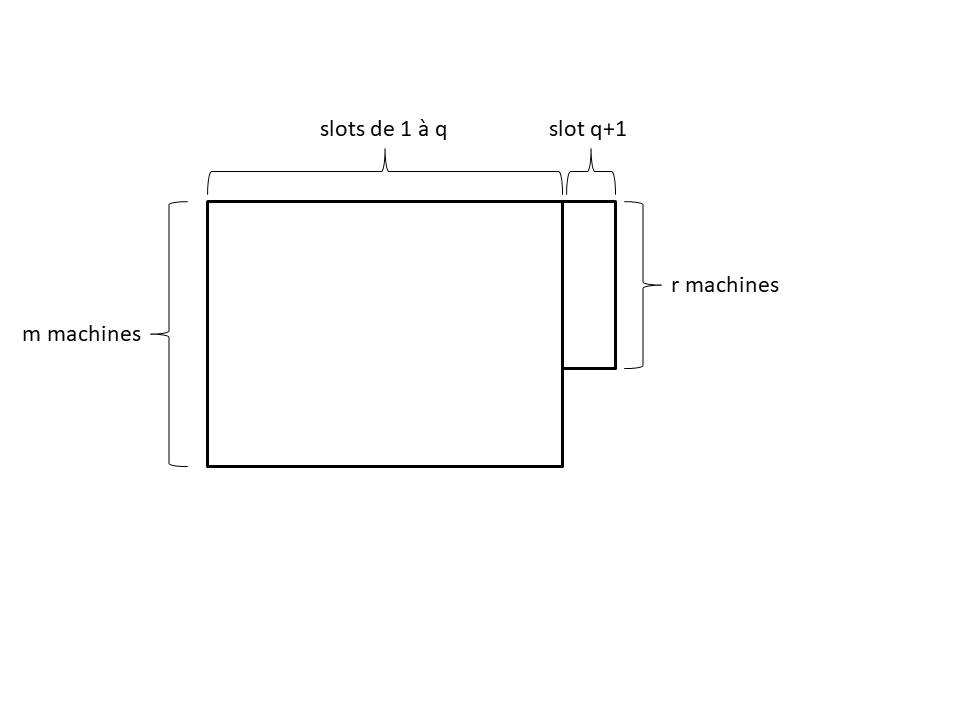
\includegraphics[scale = 0.6]{somme_opt.jpg}
\end{figure}
L'ordonnancement de la figure précédente est optimal et contient $mq+r = nx$ slots. De plus la somme des dates de fins de cet ordonnancement vaut : $m\sum\limits_{i=1}^q i +r(q+1)$.
\end{proof}
\subsection{Ordonnancement sans-envi quand tous les agents veulent minimiser $\sum C_i$}
\noindent
On pose : $n = 2mq_n+r_n$ et $x = 2mq_x+r_x$.
\begin{prop}
Si $r_nr_x=2mq'+m$, il existe un ordonnancement sans-envie et Pareto-optimal.
\end{prop}
\begin{proof}
$nx = 4m^2q_nq_x+2mq_nr_x+2mq_xr_n+r_nr_x=m(2q_xn+2q_nr_x+2q'+1)$\\
\begin{align*}
\sum C_i &= m(2q_xn+2q_nr_x+2q'+1)(q_xn+q_nr_x+q'+1)\\
&= n[2q_x(q_xn+q_nr_x+q'+1) + q_x(2q_nr_x+2q'+1)] + (2mq_nr_x+2mq'+m)(q_nr_x+q'+1)\\
&=n[2q_x(q_xn+q_nr_x+q'+1) + q_x(2q_nr_x+2q'+1)] + (2mq_nr_x+r_nr_x)(q_nr_x+q'+1)\\
&=n[2q_x(q_xn+q_nr_x+q'+1) + q_x(2q_nr_x+2q'+1)] + nr_x(q_nr_x+q'+1)\\&=n[2q_x(q_xn+q_nr_x+q'+1) + q_x(2q_nr_x+2q'+1) + r_x(q_nr_x+q'+1)]\\
\end{align*}
Il exitste donc un ordonnancement sans-envie et Pareto-optimal.
\end{proof}
\begin{prop}
Si $r_nr_x=2mq'$, il existe un ordonnancement sans-envie et Pareto-optimal ssi on n'a pas $n$ pair et $x$ impair.
\end{prop}
\begin{proof}
$nx = 4m^2q_nq_x+2mq_nr_x+2mq_xr_n+r_nr_x=m(2q_xn+2q_nr_x+2q')$\\
\begin{align*}
\sum C_i &= m(2q_xn+2q_nr_x+2q'+1)(q_xn+q_nr_x+q')\\
&= n[2q_x(q_xn+q_nr_x+q')+q_x(2q_nr_x+2q'+1)] + (2mq_nr_x+2mq'+m)(q_nr_x+q')\\
&= n[2q_x(q_xn+q_nr_x+q')+q_x(2q_nr_x+2q'+1)] + (2mq_nr_x+r_nr_x+m)(q_nr_x+q')\\
&= n[2q_x(q_xn+q_nr_x+q')+q_x(2q_nr_x+2q'+1)] + (nr_x+m)(q_nr_x+q')\\
&= n[2q_x(q_xn+q_nr_x+q')+q_x(2q_nr_x+2q'+1)+r_x(q_nr_x+q')] + mq_nr_x+q'\\
&= n[2q_x(q_xn+q_nr_x+q')+q_x(2q_nr_x+2q'+1)+r_x(q_nr_x+q')] + \dfrac{nr_x}{2}\\
\end{align*}
Si $r_x$ est pair, $\sum C_i = = n[2q_x(q_xn+q_nr_x+q')+q_x(2q_nr_x+2q'+1)+r_x(q_nr_x+q') + \dfrac{r_x}{2}]$.
Si $r_x$ est pair alors $x$ est pair.
Si $x$ est pair, il existe un ordonnancement sans-envie et Pareto-optimal.\\
Si $r_x$ est impair, alors $x$ est impair. Comme $nx$ est pair, $n$ est pair.\\
$r_x = 2p+1$\\
$\sum C_i = n[2q_x(q_xn+q_nr_x+q')+q_x(2q_nr_x+2q'+1)+r_x(q_nr_x+q') +p] + \dfrac{n}{2}$\\
Il n'existe donc pas d'ordonnancement sans-envie et Pareto-optimal.
\end{proof}

\begin{prop}
Il existe un ensemble de slots tels qu'il peut exister un ordonnancement qui permet à chaque agent d'avoir un coût de $\lceil\frac{\sum C_i}{n}\rceil$.
\end{prop}
\begin{proof}
On pose $nx = mq+r$ et $\sum C_i = nq_1+r_1$. Si $\sum C_i$ n'est pas multiple de $n$ i.e. $r_1 \neq 0$ : on décale le dernier slot de $n-r_1$\\
\begin{itemize}
\item $r = 0$ : $\sum C_i + (q+n-r_1)-q = nq_1 + r_1 + n - r_1 = n(q_1 + 1) = n\lceil\frac{\sum C_i}{n}\rceil$
\item $r \neq 0$ : $\sum C_i + (q+1+n-r_1)-(q+1) = nq_1 + r_1 + n - r_1 = n(q_1 + 1) = n\lceil\frac{\sum C_i}{n}\rceil$
\end{itemize}
\end{proof}

\section{Algorithme}
\subsection{Round-Robin}
\noindent
On considère que tous les agents ont au moins deux tâches.\\
L'algorithme fonctionne de la façon suivante :
\begin{itemize}
	\item Chaque agent donne pour chacune de ses tâches un coût aux différents slots.
	\item On définit un ordre $p$ des agents.
	\item A chaque tour, chaque agent choisit le slot qui lui coûte le moins.
\end{itemize}

\begin{exemple}
On considère une instance avec deux machines et trois agents $A$, $B$, et $D$. Les agents $A$ et $B$ veulent minimiser $\sum T_i$ et l'agent $D$ veut minimiser $\sum C_i$. Chaque agent a trois tâches à executer. On note $A_i$ (resp. $B_i$ et $D_i$) la tâche $i$ de l'agent $A$ (reps. $B$ et $D$) pour $i\in \{1, 2, 3\}$. Chaque tâche a une deadline : $d_1^A = 3$, $d_2^A = 1$, $d_2^A = 1$, $d_1^B = 1$, $d_2^B = 2$, $d_3^B = 3$, $d_1^D = 2$, $d_2^D = 4$, et $d_3^D = 4$. On considère l'ordre suivant : $DBA$. En cas d'égalité des coûts on considère les règles suivantes : 
\begin{itemize}
\item[1] on choisit la tâche qui a la plus petite deadline
\item[2] on choisit la tâche qui a l'indice le plus petit
\item[3] on choisit le slot le plus proche de la dealine
\item[4] on choisit la machine avec l'indice le plus petit.
\end{itemize}
Le tableau des coûts est le suivant :

\begin{table}[H]
    \begin{tabular}{|c||c|c|c|c|c||c|c|c|c|}
        \hline
        & $s_1^1$ & $s_2^1$ & $s_3^1$ & $s_4^1$ & $s_5^1$ & $s_1^2$ & $s_2^2$ & $s_3^2$ & $s_4^2$ \\
        \hline 
        $A_1$ & 0 & 0 & 0 & 1 & 2 & 0 & 0 & 0 & 1 \\
        $A_2$ & 0 & 1 & 2 & 3 & 4 & 0 & 1 & 2 & 3 \\
        $A_3$ & 0 & 1 & 2 & 3 & 4 & 0 & 1 & 2 & 3 \\
        \hline
        $B_1$ & 0 & 1 & 2 & 3 & 4 & 0 & 1 & 2 & 3 \\
        $B_2$ & 0 & 0 & 1 & 2 & 3 & 0 & 0 & 1 & 2 \\
        $B_3$ & 0 & 0 & 0 & 1 & 2 & 0 & 0 & 0 & 1 \\
        \hline
        $D_1$ & 1 & 2 & 3 & 4 & 5 & 1 & 2 & 3 & 4 \\
        $D_2$ & 1 & 2 & 3 & 4 & 5 & 1 & 2 & 3 & 4 \\
        $D_3$ & 1 & 2 & 3 & 4 & 5 & 1 & 2 & 3 & 4 \\
        \hline
    \end{tabular}
\end{table}

Tour 1 : 
\begin{itemize}
\item Agent $D$ : les slots qui lui coûtent le moins sont $s_1^1$ et $s_1^2$ pour chacune de ses tâches. Il choisit donc d'affecter $D_1$ au slot $s_1^1$.
\item Agent $B$ : les slots qui lui coûtent le moins sont $s_1^2$ pour $B_1$, $s_2^1$, $s_1^2$ et $s_2^2$ pour $B_2$, et $s_2^1$, $s_3^1$, $s_1^2$, $s_2^2$ et $s_3^2$ pour $B_3$. Il choisit donc d'affecter $B_1$ au slot $s_1^2$.
\item Agent $A$ : les slots qui lui coûtent le moins sont $s_2^1$, $s_3^1$, $s_2^2$ et $s_3^2$ pour $A_1$. Il choisit donc d'affecter $A_1$ au slot $s_3^1$
\end{itemize}
\begin{ganttchart}[inline]{1}{10}
    \ganttbar{$D_1$}{1}{2} 
    \ganttbar{}{3}{4} 
    \ganttbar{$A_1$}{5}{6}
    \ganttbar{}{7}{8} 
    \ganttbar{}{9}{10}\\
    \ganttbar{$B_1$}{1}{2} 
    \ganttbar{}{3}{4} 
    \ganttbar{}{5}{6} 
    \ganttbar{}{7}{8} 
\end{ganttchart}\\
\noindent
Tour 2 :
\begin{itemize}
\item Agent $D$ : les slots qui lui coûtent le moins sont $s_2^1$ et $s_2^2$ pour $D_2$ et $D_3$. Il choisit donc d'affecter $D_2$ au slot $s_2^1$.
\item Agent $B$ : les slots qui lui coûtent le moins sont $s_2^2$ pour $B_2$, et $s_2^2$ et $s_3^2$ pour $B_3$. Il choisit donc d'affecter $B_2$ au slot $s_2^2$.
\item Agent $A$ : le slot qui lui coûtent le moins est $s_3^2$ pour $A_2$ et $A_3$. Il choisit donc d'affecter $A_2$ au slot $s_3^2$
\end{itemize}
\begin{ganttchart}[inline]{1}{10}
    \ganttbar{$D_1$}{1}{2} 
    \ganttbar{$D_2$}{3}{4} 
    \ganttbar{$A_1$}{5}{6}
    \ganttbar{}{7}{8} 
    \ganttbar{}{9}{10}\\
    \ganttbar{$B_1$}{1}{2} 
    \ganttbar{$B_2$}{3}{4} 
    \ganttbar{$A_2$}{5}{6} 
    \ganttbar{}{7}{8} 
\end{ganttchart}\\
\noindent
Tour 3 :
\begin{itemize}
\item Agent $D$ : les slots qui lui coûtent le moins sont $s_4^1$ et $s_4^2$. Il choisit donc d'affecter $D_3$ au slot $s_4^1$.
\item Agent $B$ : le slot qui lui coûtent le moins est $s_4^2$. Il choisit donc d'affecter $B_3$ au slot $s_4^2$.
\item Agent $A$ : le seul slot restant est $s_5^1$. Il choisit donc d'affecter $A_3$ au slot $s_5^1$.
\end{itemize}
\begin{ganttchart}[inline]{1}{10}
    \ganttbar{$D_1$}{1}{2} 
    \ganttbar{$D_2$}{3}{4} 
    \ganttbar{$A_1$}{5}{6}
    \ganttbar{$D_3$}{7}{8} 
    \ganttbar{$A_3$}{9}{10}\\
    \ganttbar{$B_1$}{1}{2} 
    \ganttbar{$B_2$}{3}{4} 
    \ganttbar{$A_2$}{5}{6} 
    \ganttbar{$B_3$}{7}{8} 
\end{ganttchart}\\

L’ordonnancement obtenu est sans-envie up to one job : 
\begin{itemize}
\item Agent $A$ : $f_A(\sigma(A)) = 6$, $f_A(\sigma(B)) = 4$ et $f_A(\sigma(D)) = 4$. Mais si on lui retire $A_3$  : $f_A(\sigma(\{A_1,A_2\})) = 2$.
\item Agent $B$ : $f_B(\sigma(B)) = 1$, $f_B(\sigma(A)) = 5$ et $f_B(\sigma(D)) = 1$.
\item Agent $D$ : $f_D(\sigma(D)) = 7$, $f_D(\sigma(A)) = 11$ et $f_D(\sigma(B)) = 7$.
\end{itemize}

\end{exemple}

\begin{prop}
Cet algorithme est sans-envie up to one job si les coûts sont positifs et que les agents considèrent soit le coût maximal, soit la somme des coûts.
\end{prop}

\begin{proof}
Soit $p$ un ordre sur les agents. Soient $i, j \in \{1, \dots, n\}$. On note $s_i^t$ le slot alloué à l'agent $i$ au tour $t$ et $J^i_t$ la tâche associée, pour $t\in\{1,\dots,x\}$. On note $\sigma$ l'ordonnancement obtenu avec l'algorithme présenté dans cette partie.\\
\textbf{Cas 1 : $i<j$}\\
A chaque tour, $p(i)$ choisi le slot libre le moins coûteux pour lui avant $p(j)$ :\\
 $\forall t\in \{1, \dots, x\}, f_{p(i)}(s^t_{p(i)}, J^t_{p(i)})\leq f_{p(i)}(s^t_{p(j)}, J^t_{p(i)})$\\
 Si $i$ considère le coût maximal : $f_{p(i)}(\sigma(i)) = \max\limits_{t = 1}^x f_{p(i)}(s^t_{p(i)}, J^t_{p(i)}) \leq f_{p(i)}(\sigma(j)) = \max\limits_{t = 1}^x f_{p(i)}(s^t_{p(j)}, J^t_{p(i)})$\\
 Si $i$ considère la somme des coûts : $f_{p(i)}(\sigma(i)) = \sum\limits_{t = 1}^x f_{p(i)}(s^t_{p(i)}, J^t_{p(i)})\leq f_{p(i)}(\sigma(j)) = \sum\limits_{t = 1}^x f_{p(i)}(s^t_{p(j)}, J^t_{p(i)})$\\
\textbf{Cas 2 : $i>j$}\\
Soit $t\in\{1,\dots,x-1\}$.\\
Le slot alloué à $p(i)$ au tour $t$ lui coûte moins que le slot alloué à $p(j)$ au tour $t+1$ : \\
$f_{p(i)}(s^t_{p(i)}, J^t_{p(i)})\leq f_{p(i)}(s^{t+1}_{p(j)}, J^{t+1}_{p(i)})$\\
Si $i$ considère le coût maximal : \\
$f_{p(i)}(\sigma(J^{p(i)}\backslash\{J_{p(i)}^x\})) = \max\limits_{t = 1}^{x-1} f_{p(i)}(s^t_{p(i)}, J^t_{p(i)}) = f_{p(i)}(s^{x-1}_{p(i)}, J^{x-1}_{p(i)}) \leq f_{p(i)}(s^x_{p(j)}, J^x_{p(i)}) = f_{p(i)}(\sigma(j))$\\
Si $i$ considère la somme des coûts : \\
$f_{p(i)}(\sigma(J^{p(i)}\backslash\{J_{p(i)}^x\})) = \sum\limits_{t = 1}^{x-1} f_{p(i)}(s^t_{p(i)}, J^t_{p(i)}) \leq \sum\limits_{t = 2}^{x} f_{p(i)}(s^t_{p(j)}, J^t_{p(i)}) \leq \sum\limits_{t = 1}^{x} f_{p(i)}(s^t_{p(j)}, J^t_{p(i)}) = f_{p(i)}(\sigma(j))$.
\end{proof}

\subsubsection{Round-Robin 2eme version}
\noindent
On considère que tous les agents ont au moins deux tâches.\\
L'algorithme fonctionne de la façon suivante :
\begin{itemize}
	\item Chaque agent attribut un vecteur coût aux différents slots.
	\item On définit un ordre $p$ des agents.
	\item A chaque tour, chaque agent choisit le slot qui lui coûte le moins.
\end{itemize}

\begin{prop}
Cet algorithme est sans-envie up to one job si tous les vecteurs coûts sont comparables soit le coût maximal, soit la somme des coûts.
\end{prop}

\begin{proof}
Soit $p$ un ordre sur les agents. Soient $i, j \in \{1, \dots, n\}$. On note $s_i^t$ le slot alloué à l'agent $i$ au tour $t$ et $J^i_t$ la tâche associée, pour $t\in\{1,\dots,x\}$. On note $\sigma$ l'ordonnancement obtenu avec l'algorithme présenté dans cette partie.\\
\textbf{Cas 1 : $i<j$}\\
A chaque tour, $p(i)$ choisi le slot libre le moins coûteux pour lui avant $p(j)$ :\\
 $\forall t\in \{1, \dots, x\}, f_{p(i)}(s^t_{p(i)}, J^t_{p(i)})\leq f_{p(i)}(s^t_{p(j)}, J^t_{p(i)})$\\
 Si $i$ considère le coût maximal : $f_{p(i)}(\sigma(i)) = \max\limits_{t = 1}^x f_{p(i)}(s^t_{p(i)}, J^t_{p(i)}) \leq f_{p(i)}(\sigma(j)) = \max\limits_{t = 1}^x f_{p(i)}(s^t_{p(j)}, J^t_{p(i)})$\\
 Si $i$ considère la somme des coûts : $f_{p(i)}(\sigma(i)) = \sum\limits_{t = 1}^x f_{p(i)}(s^t_{p(i)}, J^t_{p(i)})\leq f_{p(i)}(\sigma(j)) = \sum\limits_{t = 1}^x f_{p(i)}(s^t_{p(j)}, J^t_{p(i)})$\\
\textbf{Cas 2 : $i>j$}\\
Soit $t\in\{1,\dots,x-1\}$.\\
Le slot alloué à $p(i)$ au tour $t$ lui coûte moins que le slot alloué à $p(j)$ au tour $t+1$ : \\
$f_{p(i)}(s^t_{p(i)}, J^t_{p(i)})\leq f_{p(i)}(s^{t+1}_{p(j)}, J^{t+1}_{p(i)})$\\
Si $i$ considère le coût maximal : \\
$f_{p(i)}(\sigma(J^{p(i)}\backslash\{J_{p(i)}^x\})) = \max\limits_{t = 1}^{x-1} f_{p(i)}(s^t_{p(i)}, J^t_{p(i)}) = f_{p(i)}(s^{x-1}_{p(i)}, J^{x-1}_{p(i)}) \leq f_{p(i)}(s^x_{p(j)}, J^x_{p(i)}) = f_{p(i)}(\sigma(j))$\\
Si $i$ considère la somme des coûts : \\
$f_{p(i)}(\sigma(J^{p(i)}\backslash\{J_{p(i)}^x\})) = \sum\limits_{t = 1}^{x-1} f_{p(i)}(s^t_{p(i)}, J^t_{p(i)}) \leq \sum\limits_{t = 2}^{x} f_{p(i)}(s^t_{p(j)}, J^t_{p(i)}) \leq \sum\limits_{t = 1}^{x} f_{p(i)}(s^t_{p(j)}, J^t_{p(i)}) = f_{p(i)}(\sigma(j))$.
\end{proof}

\subsection{Ordonnancement sans-envi quand $m = 1$ et que tous les agents veulent minimiser $\sum C_i$}
\noindent
Dans cette section, on présente un algorithme qui renvoie un ordonnancement sans-envie quand $m = 1$ et que tous les agents veulent minimiser $\sum C_i$. On considère que $n\geq 2$ et $x\geq 2$.\\
\begin{itemize}
\item \textbf{$x$ pair :} on répète la séquence suivante $\dfrac{x}{2}$ fois : \\
\begin{ganttchart}[inline]{1}{12}
    \ganttbar{$a_1$}{1}{2}
    \ganttbar{$\dots$}{3}{4} 
    \ganttbar{$a_n$}{5}{6} 
    \ganttbar{$a_n$}{7}{8} 
    \ganttbar{$\dots$}{9}{10}
    \ganttbar{$a_1$}{11}{12} 
\end{ganttchart}
\begin{exemple}
$n=3$ et $x=4$. On note les agents $a$, $b$ et $c$.\\
\begin{ganttchart}[inline]{1}{24}
    \ganttbar{$a$}{1}{2}
    \ganttbar{$b$}{3}{4} 
    \ganttbar{$c$}{5}{6} 
    \ganttbar{$c$}{7}{8} 
    \ganttbar{$b$}{9}{10}
    \ganttbar{$a$}{11}{12} 
    \ganttbar{$a$}{13}{14}
    \ganttbar{$b$}{15}{16} 
    \ganttbar{$c$}{17}{18} 
    \ganttbar{$c$}{19}{20} 
    \ganttbar{$b$}{21}{22}
    \ganttbar{$a$}{23}{24} 
\end{ganttchart}\\
Chaque agent a un coût de 26. Cet ordonnancement est sans-envi.
\end{exemple}
\begin{prop}
L'ordonnancement obtenu est sans-envi
\end{prop}
\begin{proof}
La somme des dates de fin de tous les slots qui seront alloués est :\\$\sum\limits_{i=1}^{nx} i = n\dfrac{x}{2}(nx + 1)$. Pour que l'ordonnancement soit sans-envi, il faut que le coût de l'ordonnancement pour chaque agent soit $\dfrac{x}{2}(nx + 1)$.\\
Soit $i\in\{1,\dots,n\}$. A l'itération $j$ de la séquence, l'agent $a_i$ aura les slots $2n(j-1) + i$ et $2n(j-1) + 2n + 1 -i$. Le coût de l'agent $a_i$ à l'itération $j$ de la séquence est donc : $4n(j-1) + 2n + 1$.\\
Le coût total pour l'agent $a_i$ est :\\
 $\sum\limits_{j = 1}^{\frac{x}{2}} (4n(j-1) + 2n + 1) = 4n\dfrac{\frac{x}{2}(\frac{x}{2} - 1)}{2} + (2n + 1)\dfrac{x}{2} = nx\dfrac{x}{2} - nx + nx + \dfrac{x}{2} = \dfrac{x}{2}(nx + 1)$.\\
 Cet ordonnancement est bien sans-envi.
\end{proof}
\item \textbf{$x$ impair et $n$ impair:} A partir du slot $3n + 1$, on répète la séquence suivante $\dfrac{x-3}{2}$ fois :
\begin{ganttchart}[inline]{1}{12}
    \ganttbar{$a_1$}{1}{2}
    \ganttbar{$\dots$}{3}{4} 
    \ganttbar{$a_n$}{5}{6} 
    \ganttbar{$a_n$}{7}{8} 
    \ganttbar{$\dots$}{9}{10}
    \ganttbar{$a_1$}{11}{12} 
\end{ganttchart}\\
Pour les $3n$ premiers slots on considère l'allocation suivante :
\begin{itemize}
\item[•] pour $i\in \{1,\dots,\dfrac{n+1}{2} \}$ on alloue à $a_i$ les slots $3n + 1 - i$, $\dfrac{3n+3}{2} - i$, et $2i-1$.
\item[•] pour $i\in \{\dfrac{n+3}{2}\dots,n \}$ on alloue à $a_i$ les slots $3n + 1 - i$, $2i - n-1$, et $\dfrac{5n+3}{2}-i$.
\end{itemize}
\begin{exemple}
$n=3$ et $x=5$. On note les agents $a$, $b$ et $c$.\\
\begin{ganttchart}[inline]{1}{30}
    \ganttbar{$a$}{1}{2}
    \ganttbar{$c$}{3}{4} 
    \ganttbar{$b$}{5}{6} 
    \ganttbar{$b$}{7}{8} 
    \ganttbar{$a$}{9}{10}
    \ganttbar{$c$}{11}{12} 
    \ganttbar{$c$}{13}{14}
    \ganttbar{$b$}{15}{16} 
    \ganttbar{$a$}{17}{18} 
    \ganttbar{$a$}{19}{20} 
    \ganttbar{$b$}{21}{22}
    \ganttbar{$c$}{23}{24} 
    \ganttbar{$c$}{25}{26}
    \ganttbar{$b$}{27}{28} 
    \ganttbar{$a$}{29}{30} 
\end{ganttchart}\\
Chaque agent a un coût de 40. Cet ordonnancement est sans-envi.
\end{exemple}
\begin{prop}
L'ordonnancement est valide et sans-envi.
\end{prop}
\begin{proof}
Soit $i\in\{1,\dots,n\}$.\\
Montrons que l'allocation des $3n$ premiers slots est valide (aucun slot n'est alloué deux fois et tous les slots sont alloués).
\begin{itemize}
\item[•] pour les slots $\{1,\dots,n\}$ :\\
\begin{tabular}{ccc}
$1\leq i \leq \dfrac{n+1}{2}$ & & $\dfrac{n+3}{2}\leq i \leq n$\\
$2\leq 2i \leq n+1$ & & $n+3\leq 2i\leq 2n$\\
$1\leq 2i-1\leq n$ & & $2\leq 2i - n-1\leq n-1$\\
ensemble des entiers impairs entre 1 et $n$ & & ensemble des entiers pairs entre 1 et $n$
\end{tabular}\\
Entre 1 et $n$, tous les slot sont alloués exactement une fois.
\item[•] pour les slots $\{n+1,\dots,2n\}$ :\\
\begin{tabular}{ccc}
$1\leq i \leq \dfrac{n+1}{2}$ & & $\dfrac{n+3}{2}\leq i \leq n$\\
$-\dfrac{n+1}{2}\leq -i\leq -1$ & & $-n\leq -i \leq -\dfrac{n+3}{2}$\\
$n+1\leq -i+\dfrac{3n+3}{2}\leq \dfrac{3n+1}{2}$ & & $\dfrac{3n+3}{2}\leq -i+\dfrac{5n+3}{2} \leq 2n$\\
ensemble des entiers entre $n+1$ et $\dfrac{3n+1}{2}$ & & ensemble des entiers entre $\dfrac{3n+3}{2}$ et $2n$
\end{tabular}\\
Entre $n+1$ et $2n$, tous les slot sont alloués exactement une fois.
\item[•] pour les slots $\{2n+1,\dots,3n\}$ :\\
\begin{tabular}{ccc}
$1\leq i \leq \dfrac{n+1}{2}$ & & $\dfrac{n+3}{2}\leq i \leq n$\\
$-\dfrac{n+1}{2}\leq -i\leq -1$ & & $-n\leq -i \leq -\dfrac{n+3}{2}$\\
$\dfrac{5n+1}{2}\leq 3n+1-i\leq 3n$ & & $2n+1\leq 3n+1-i \leq \dfrac{5n-1}{2}$\\
ensemble des entiers entre $\dfrac{5n+1}{2}$ et $3n$ & & ensemble des entiers entre $2n + 1$ et $\dfrac{5n-1}{2}$
\end{tabular}\\
Entre $2n+1$ et $3n$, tous les slot sont alloués exactement une fois.\\
\end{itemize}
Cette ordonnancement est donc valide. Montrons maintenant que l'ordonnancement est sans-envi. Nous avons montré précédemment que le coût total des slots est $n\dfrac{x}{2}(nx+1)$. Pour que l'ordonnancement soit équitable, l'ordonnancement de chaque agent doit avoir un coût de $\dfrac{x}{2}(nx+1)$.\\
Calculons le coût de l'agent $a_i$ pour les $3n$ premiers slots :
\begin{itemize}
\item[•] si $i\in \{1,\dots,\dfrac{n+1}{2}\}$, le coût pour l'agent $a_i$ si on ne considère que les $3n$ premiers slots est : \\
$3n+1-i+\dfrac{3n+3}{2}-i+2i-1 = \dfrac{9n+3}{2}$
\item[•] si $i\in \{\dfrac{n+1}{2},\dots,n\}$, le coût pour l'agent $a_i$ si on ne considère que les $3n$ premiers slots est : \\
$3n+1-i+2i-n-1+\dfrac{5n+3}{2}-i = \dfrac{9n+3}{2}$
\end{itemize}
A l'itération $j$ de la séquence 
\begin{ganttchart}[inline]{1}{12}
    \ganttbar{$a_1$}{1}{2}
    \ganttbar{$\dots$}{3}{4} 
    \ganttbar{$a_n$}{5}{6} 
    \ganttbar{$a_n$}{7}{8} 
    \ganttbar{$\dots$}{9}{10}
    \ganttbar{$a_1$}{11}{12} 
\end{ganttchart} , le coût de l'agent $a_i$ est :\\
$3n + 2n(j-1) + i + 3n + 2n(j-1) + 2n+1 -i = 4nj+4n+1$.\\
Le coût total de l'agent $a_i$ est donc :
\begin{align*}
\dfrac{9n+3}{2}+\sum\limits_{i=1}^{\frac{x-3}{2}}(4nj+4n+1) &= \dfrac{9n+3}{2} + \dfrac{x-3}{2} + 2n(x-3) + n(x-3)(\dfrac{x-3}{2}+1)\\
&= \dfrac{9n+3}{2} + (x-3)(\dfrac{1}{2} + 2n + n(\dfrac{x-3}{2}+1))\\
&= \dfrac{9n+3}{2} + (x-3)(\dfrac{3n+1}{2}+n\dfrac{x}{2})\\
&= x\dfrac{3n+1}{2} +nx\dfrac{x}{2}-3n\dfrac{x}{2}\\
&= \dfrac{x}{2}(nx +1)
\end{align*}
Cet ordonnancement est donc sans-envie.
\end{proof}
\item \textbf{$x$ impair et $n$ pair:} On retire le slot $3n + 1 - \dfrac{n}{2}$, et à partir du slot $3n + 2$, on répète la séquence suivante $\dfrac{x-3}{2}$ fois :
\begin{ganttchart}[inline]{1}{12}
    \ganttbar{$a_1$}{1}{2}
    \ganttbar{$\dots$}{3}{4} 
    \ganttbar{$a_n$}{5}{6} 
    \ganttbar{$a_n$}{7}{8} 
    \ganttbar{$\dots$}{9}{10}
    \ganttbar{$a_1$}{11}{12} 
\end{ganttchart}\\
Pour les $3n$ premiers slots on considère l'allocation suivante :
\begin{itemize}
\item[•] pour $i\in \{1,\dots,\dfrac{n}{2} \}$ on alloue à $a_i$ les slots $3n + 2 - i$, $\dfrac{3n+2}{2} - i$, et $2i-1$.
\item[•] pour $i\in \{\dfrac{n+2}{2}\dots,n \}$ on alloue à $a_i$ les slots $3n + 1 - i$, $2i - n$, et $\dfrac{5n+2}{2}-i$.
\end{itemize}
\begin{exemple}
$n=4$ et $x=5$. On note les agents $a$, $b$, $c$ et $d$.\\
\begin{ganttchart}[inline]{1}{34}
    \ganttbar{$a$}{1}{2}
    \ganttbar{$c$}{3}{4} 
    \ganttbar{$b$}{5}{6} 
    \ganttbar{$d$}{7}{8} 
    \ganttbar{$b$}{9}{10}
    \ganttbar{$a$}{11}{12} 
    \ganttbar{$d$}{13}{14}
    \ganttbar{$c$}{15}{16} 
    \ganttbar{$d$}{17}{18} 
    \ganttbar{$c$}{19}{20} 
    \ganttbar{}{21}{22}
    \ganttbar{$b$}{23}{24} 
    \ganttbar{$a$}{25}{26}
    \ganttbar{$a$}{27}{28} 
    \ganttbar{$b$}{29}{30}
    \ganttbar{$c$}{31}{32} 
    \ganttbar{$d$}{33}{34}\\
    \ganttbar{$d$}{1}{2} 
    \ganttbar{$c$}{3}{4} 
    \ganttbar{$b$}{5}{6} 
    \ganttbar{$a$}{7}{8} 
\end{ganttchart}\\
Chaque agent a un coût de 55. Cet ordonnancement est sans-envi.
\end{exemple}
\begin{prop}
L'ordonnancement est valide et sans-envi.
\end{prop}
\begin{proof}
Soit $i\in\{1,\dots,n\}$.\\
Montrons que l'allocation des $3n$ premiers slots est valide (aucun slot n'est alloué deux fois et tous les slots sont alloués).
\begin{itemize}
\item[•] pour les slots $\{1,\dots,n\}$ :\\
\begin{tabular}{ccc}
$1\leq i \leq \dfrac{n}{2}$ & & $\dfrac{n+2}{2}\leq i \leq n$\\
$2\leq 2i \leq n$ & & $n+2\leq 2i\leq 2n$\\
$1\leq 2i-1\leq n-1$ & & $2\leq 2i - n\leq n$\\
ensemble des entiers impairs entre 1 et $n$ & & ensemble des entiers pairs entre 1 et $n$
\end{tabular}\\
Entre 1 et $n$, tous les slot sont alloués exactement une fois.
\newpage
\item[•] pour les slots $\{n+1,\dots,2n\}$ :\\
\begin{tabular}{ccc}
$1\leq i \leq \dfrac{n}{2}$ & & $\dfrac{n+2}{2}\leq i \leq n$\\
$-\dfrac{n}{2}\leq -i\leq -1$ & & $-n\leq -i \leq -\dfrac{n+2}{2}$\\
$n+1 \leq \dfrac{3n}{2}+1-i\leq\dfrac{3n}{2}$ & & $\dfrac{3n+2}{2}\leq \dfrac{5n+2}{2}-i\leq 2n$\\
ensemble des entiers entre $n+1$ et $\dfrac{3n}{2}$ & & ensemble des entiers entre $\dfrac{3n+2}{2}$ et $2n$. 
\end{tabular}\\
Entre $n+1$ et $2n$, tous les slot sont alloués exactement une fois.
\item[•] pour les slots $\{2n+1,\dots,3n + 1\}$ :\\
\begin{tabular}{ccc}
$1\leq i \leq \dfrac{n}{2}$ & & $\dfrac{n+2}{2}\leq i \leq n$\\
$-\dfrac{n}{2}\leq -i\leq -1$ & & $-n\leq -i \leq -\dfrac{n+2}{2}$\\
$\dfrac{5n+4}{2}\leq 3n+2-i\leq 3n+1$ & & $2n+1\leq 3n+1-i \leq \dfrac{5n}{2}$\\
ensemble des entiers entre $\dfrac{5n+4}{2}$ et $3n$ & & ensemble des entiers entre $2n + 1$ et $\dfrac{5n}{2}$
\end{tabular}\\
Entre $2n+1$ et $3n+1$, tous les slot sont alloués exactement une fois sauf le slot $\dfrac{5n+2}{2}$.\\
\end{itemize}
Cette ordonnancement est donc valide. Montrons maintenant que l'ordonnancement est sans-envi. Déterminons dans un premier temps le coût total des slots :\\
$(\sum\limits_{i=1}^{nx+1}i)-\dfrac{5n+2}{2} = 	\dfrac{(nx+1)(nx+2)}{2}-\dfrac{5n+2}{2} = n(x\dfrac{nx+3}{2}-\dfrac{5}{2})$\\
Pour que l'ordonnancement soit sans-envi, le coût de chaque agent doit être $x\dfrac{nx+3}{2}-\dfrac{5}{2}$.\\
Calculons le coût de l'agent $a_i$ pour les $3n+1$ premiers slots :
\begin{itemize}
\item[•] si $i\in \{1,\dots,\dfrac{n+1}{2}\}$, le coût pour l'agent $a_i$ si on ne considère que les $3n$ premiers slots est : \\
$3n+2-i+\dfrac{3n+2}{2}-i+2i-1 = \dfrac{9n+4}{2}$
\item[•] si $i\in \{\dfrac{n+1}{2},\dots,n\}$, le coût pour l'agent $a_i$ si on ne considère que les $3n$ premiers slots est : \\
$3n+1-i+2i-n+\dfrac{5n+2}{2}-i = \dfrac{9n+4}{2}$
\end{itemize}
A l'itération $j$ de la séquence 
\begin{ganttchart}[inline]{1}{12}
    \ganttbar{$a_1$}{1}{2}
    \ganttbar{$\dots$}{3}{4} 
    \ganttbar{$a_n$}{5}{6} 
    \ganttbar{$a_n$}{7}{8} 
    \ganttbar{$\dots$}{9}{10}
    \ganttbar{$a_1$}{11}{12} 
\end{ganttchart} , le coût de l'agent $a_i$ est :\\
$3n + 1 + 2n(j-1) + i + 3n + 1 + 2n(j-1) + 2n+1 -i = 4nj+4n+3$.\\
Le coût total de l'agent $a_i$ est donc :
\begin{align*}
\dfrac{9n+4}{2}+\sum\limits_{i=1}^{\frac{x-3}{2}}(4nj+4n+3) &= \dfrac{9n+4}{2} + 3\dfrac{x-3}{2} + 2n(x-3) + n(x-3)(\dfrac{x-3}{2}+1)\\
&= \dfrac{9n+4}{2} + (x-3)(\dfrac{3}{2} + 2n + n(\dfrac{x-3}{2}+1))\\
&= \dfrac{9n+4}{2} + (x-3)(\dfrac{3n+3}{2}+n\dfrac{x}{2})\\
&= x\dfrac{3n+3}{2} +nx\dfrac{x}{2}-\dfrac{5}{2}-3n\dfrac{x}{2}\\
&= \dfrac{x}{2}(nx+3)-\dfrac{5}{2}
\end{align*}
Cet ordonnancement est donc sans-envie.
\end{proof}
\end{itemize}

\newpage
\bibliographystyle{unsrt}
\bibliography{ref}

\end{document}